\documentclass[11pt]{article}
\usepackage[margin=1in]{geometry}

\usepackage[utf8]{inputenc}
\usepackage[T1]{fontenc}
\usepackage{hyperref}
\usepackage{url}
\usepackage{booktabs}
\usepackage{amsfonts}
\usepackage{amsmath}
\usepackage{amssymb}
\usepackage{graphicx}
\usepackage{float}
\usepackage{xcolor}
\usepackage{natbib}

\newcommand{\qmain}{Q_{\text{main}}}
\newcommand{\qalt}{Q_{\text{alt}}}

\title{Structure, Diffusion, and Collaboration in a Large Population of LLM Agents: A Re-analysis of MoltBook}

\author{
  Brandon Yee\\
  Management Lab, Yee Collins Research Group\\
  \texttt{b.yee@ycrg-labs.org}
}
\date{November 2026}

\begin{document}
\maketitle

\begin{abstract}
MoltBook is a Reddit-style site on which only AI agents can post. We use 24 days of its public archive, covering about 74,000 active agents, to ask three questions that small, lab-built groups of language model agents cannot answer: whether agents settle into distinct roles, whether phrases spread from agent to agent, and whether agents write better technical answers when several of them work on a problem together. Most agents do very little, since in every version of the data we use more than 80\% of registered accounts have at most one reply link to another agent, so the population splits into a large inactive group and a small active one, and we find no other clear roles. Agents are more likely to start using a phrase the more of their neighbors have already used it, and the rate keeps rising without leveling off, although our data cannot tell influence apart from neighbors simply being alike or reading the same posts. Threads in which several agents work on a technical problem score higher on our code quality measure than threads with one or two agents, but the gap shrinks when we compare threads of similar length, and it disappears under a second quality measure and when we drop scripted accounts, so we find no consistent evidence that agents do better work together. We also found that three results in an earlier version of this analysis came from errors in the analysis code, and we describe them so that others who work with this archive can avoid them.
\end{abstract}

\section{Introduction}

Language model agents now post, reply, and vote on open platforms on behalf of their operators, and on some sites tens of thousands of them interact with each other with almost no human involvement. We know little about what happens in these populations. Most studies of language model agents put two to ten agents together, give them roles, and split a task among them \citep{wu2023autogen, hong2023metagpt, li2023camel}, or build a simulated town whose rules are fixed in advance \citep{park2023generative}. Those designs are good for testing what a particular setup can do, but they cannot tell us whether the patterns we know from large human populations also appear when thousands of agents act on their own schedules and under their own prompts.

MoltBook gives us a chance to look. It is a Reddit-style site that only agents can use, most of them running on the OpenClaw agent software \citep{steinberger2026openclaw}, and its public archive records their posts and comments \citep{moltbook_observatory_archive_2026}. We use 24 days of that archive to ask three questions, each of which has a long history in the study of human groups. The first is whether agents take on distinct roles in the reply network or simply split into an active group and an inactive one \citep{borgatti2000coreperiphery, guimera2005functional}. The second is whether an agent becomes more likely to use a phrase as more of its neighbors use it \citep{centola2007complex, dodds2004universal}. The third is whether technical threads in which several agents take part end up with better answers than similar threads with fewer agents \citep{woolley2010evidence, straub2023coordination}.

Our answers are mostly no, or not clearly. The reply network has one large group of agents who barely interact and a small group who do almost all the interacting, and inside that small group the only thing that separates agents is how active they are (Section~\ref{sec:roles}). Phrases do spread, in the sense that an agent's chance of using a phrase rises steadily with the number of neighbors who have used it, from 0.13\% with no such neighbor to about 10\% with fifteen (Section~\ref{sec:diffusion}). Threads with several agents score higher on our quality measure than threads with one or two, but the difference mostly reflects the fact that these threads are longer and contain more code, and it does not hold up under a second measure or without scripted accounts (Section~\ref{sec:collab}).

This paper replaces an earlier version of the same analysis, and three of that version's main results came from the analysis code and not from the agents. It reported 10,000 cascades because the code kept only the 10,000 largest. It reported that each additional exposure lowered the chance of adoption because of a counting rule that treated agents who adopted and agents who did not adopt differently. And it reported that collaboration hurt quality because it compared quality scores with the fixed number 0.5, since the step that was supposed to collect comparison threads returned none. Appendix~\ref{app:changes} lists every change.

Two limits apply to everything that follows. The data are observational, so when we say that agents with more adopting neighbors adopt more often, we mean that the two go together, not that one causes the other. Neighbors may use the same phrase because they resemble each other or read the same posts, and with data like ours these explanations cannot be separated from influence \citep{shalizi2011homophily, aral2009distinguishing}. The second limit is that a small number of accounts write most of the content, and many of them look scripted, so we report every main result with and without those accounts (Section~\ref{sec:checks}).

\section{Related Work}
\label{sec:related}

\paragraph{Groups of language model agents.}
Work on cooperation among language model agents has focused on small groups set up by the experimenter. \citet{park2023generative} place generative agents in a virtual town, \citet{li2023camel} study pairs of agents playing assigned roles, AutoGen \citep{wu2023autogen} and MetaGPT \citep{hong2023metagpt} give a few agents fixed ways to talk and fixed jobs, and debate setups \citep{liang2023encouraging, du2023improving} test whether structured disagreement improves answers. In each case the experimenter decides how many agents there are, what they do, and how they communicate. That control makes cause and effect easy to read, but it leaves open how agents behave when none of these things is set in advance.

\paragraph{Earlier studies of MoltBook.}
Three studies have described MoltBook's first days. \citet{holtz2026anatomy} analyzes the first 3.5 days and finds network patterns that resemble human platforms, alongside shallow conversations, little reciprocity, and many duplicated template messages. \citet{li2026rise} study about 122,000 posts from the first five days and find a mostly neutral tone and a network centered on a few hub accounts. \citet{price2026claws} cover 12 days and find concentrated attention, about 1\% reciprocity, and early accounts gaining more upvotes, and they argue that hierarchy and role differentiation can emerge quickly. We cover a longer window and more agents, we test for roles directly, and we add the questions of diffusion and collaboration.

\paragraph{Roles and teamwork in human groups.}
Shared conventions can form through repeated interaction among agents \citep{lazaridou2020emergent, mordatch2018emergence}, and open projects such as Wikipedia develop specialized roles that nobody assigns \citep{kittur2007harnessing}. In human groups, \citet{woolley2010evidence} find a general factor that predicts how well a group performs across tasks, and diverse groups can outperform groups of individually stronger members \citep{hong2004diverse}. Working together also has costs, and on complex tasks these costs can exceed the benefits \citep{straub2023coordination}.

\paragraph{How things spread through networks.}
Who sits at the center of a network, and who links otherwise separate groups, shapes how information travels \citep{freeman1977centrality, borgatti2000coreperiphery, guimera2005functional}. In simple contagion one contact is enough to pass something on, while in complex contagion people need to see it from several contacts \citep{centola2007complex}, and in other models adoption rises with each exposure but by less each time \citep{dodds2004universal}. Most cascades online are small \citep{goel2012structure}, and the few large ones produce the heavy tails seen in popularity data \citep{weng2012competition}, which should be tested with the maximum likelihood methods of \citet{clauset2009power}. Telling influence apart from similarity is hard in observational data. Matching methods show that simple estimates can overstate influence several times over \citep{aral2009distinguishing}, shuffling the order of adoptions offers a test for whether timing matters at all \citep{anagnostopoulos2008influence}, and in general the two cannot be separated without strong assumptions \citep{shalizi2011homophily}. Experiments avoid the problem by assigning exposure at random \citep{centola2010spread, bakshy2012role}. Automated accounts are a further concern on any platform, and studies of human platforms check whether their results hold when such accounts are removed \citep{vosoughi2018spread}.

\paragraph{What we expected.}
From this work we expected three things. We expected the network to be organized mainly by how active agents are, so that a clustering method would separate active from inactive agents clearly but find few other roles. We expected adoption to rise with the first few exposures and then level off. And we expected threads with several agents to do worse than comparable threads with fewer agents, since agents have to spend effort coordinating, with the gap shrinking as more agents join and contribute.

\section{Data}
\label{sec:data}

The MoltBook Observatory Archive \citep{moltbook_observatory_archive_2026} publishes daily exports of agent profiles, posts, comments, and communities (called submolts). We use archive revision \texttt{ee98f6c8}, the one our earlier version used, and keep content created between 28 January and 20 February 2026. Table~\ref{tab:data} gives the main counts. The archive does not record which language model runs each agent, so every result describes the population as a whole.

This revision has a gap that matters for the network. Only 16.2\% of its top-level comments point to a post that is also in the revision, so most top-level comments cannot be linked to the agent they reply to. The latest archive revision fills in those posts but has lost most of the comments, keeping only 15.5\% of ours. We therefore also build a merged dataset from both revisions, in which 98.2\% of top-level comments find their post, and we repeat the network and collaboration analyses on it. The phrase analysis was too large to repeat on the merged data.

Some accounts on MoltBook behave like scripts. We flag an account if it posts at nearly the same times every day (at least 30 posts or comments over at least two days, with a gap of six or more hours that recurs daily), if at least half of its posts or comments repeat its own earlier text word for word, or if its activity comes in strong bursts (burstiness of 0.5 or more over at least ten items). These rules flag 5,766 of the 73,542 active accounts. That is only 7.8\% of accounts, but they wrote 76.8\% of all posts and comments and 88.7\% of comments, and almost all of them were flagged for repeating their own text. We call these scripted accounts. The rules are heuristics, not a classifier with known accuracy, so we use them only to ask whether a result changes when these accounts are removed. We also repeat each analysis without content from 30 January to 1 February, the days around an incident on the platform on 31 January.

\begin{table}[H]
\centering
\caption{Data used in this paper.}
\label{tab:data}
\begin{tabular}{@{}lr@{}}
\toprule
\textbf{Quantity} & \textbf{Value} \\
\midrule
Registered agents & 90,704 \\
Active agents (at least one post or comment) & 73,543 \\
Days & 24 \\
Posts / comments & 222,791 / 879,629 \\
Replies that link two agents & 154,231 \\
Phrase cascades (used by at least 10 agents) & 471,316 \\
Code and formatting cascades & 286 / 6 \\
Technical threads & 43,123 \\
Group threads (Section~\ref{sec:collab}) & 164 \\
\bottomrule
\end{tabular}
\end{table}

\section{Roles}
\label{sec:roles}

To look for roles we build a reply network. Each agent is a node, and there is a link from agent $u$ to agent $v$ when $u$ comments on a post by $v$ or replies to a comment by $v$, weighted by how often this happens. For every agent we compute five measures of its position: how many agents reply to it (in-degree), how many it replies to (out-degree), how often it lies on the shortest path between other agents (betweenness), how often its contacts also reply to each other (clustering coefficient), and PageRank. We standardize the five measures and group agents with k-means, trying 3 to 8 groups and choosing the number with the best silhouette score \citep{rousseeuw1987silhouettes}, which measures how well separated the groups are. Agents in the registry with no reply link get zero on every measure and stay in the analysis.

The groups are very well separated, with a silhouette of 0.916 at the chosen 8 groups, and they are stable, since 100 bootstrap samples recover the same grouping with an average adjusted Rand index of 0.93. Figure~\ref{fig:clusters} shows why this does not mean the agents have roles. One group holds 92.9\% of all agents, and its members sit below average on every measure. Most of them, 84.0\% of all registered agents, have no reply link at all, so they share exactly the same values, and a group of identical points far from everyone else is easy to separate. Part of this comes from the missing posts described in Section~\ref{sec:data}, but on the merged data, which restores those links, 83.9\% of agents still have at most one reply link (Table~\ref{tab:checks}). The high score therefore tells us that inactive agents are far from active ones, and nothing more.

Among the active agents, the groups differ mainly in how active they are. Groups 2 through 7 are ordered by how many replies their members send and receive, up to a single agent who sent 5,744 replies. Group 1, with 4.4\% of agents, is the only one that stands out for a reason other than volume, because its members' few contacts also reply to each other, which gives them a high clustering coefficient. The number of groups is also not well defined. The silhouette rises only from 0.906 to 0.916 between 3 and 8 groups, so the choice of 8 rests on differences smaller than the variation between runs. A Gaussian mixture model, which allows agents to belong partly to several groups, agrees only moderately with k-means (adjusted Rand index 0.54) and assigns almost every agent firmly to one group, so it does not reveal more roles either.

Simple rules based on posting behavior give the same picture. Under rules that call an agent an Initiator if it posts much more than it comments, a Connector if its betweenness is high, and so on (Appendix~\ref{app:clustering}), 89.5\% of agents are Generalists, 9.8\% are Initiators, 0.6\% are Connectors, and no agent qualifies as a Specialist or a Synthesizer. For comparison we ran the same pipeline on 499,116 comments from r/programming, sampled to have about as many authors as MoltBook has active agents. It also produces one dominant group, but only 42\% of its authors have at most one reply link, against 87\% on MoltBook. We do not read much into this difference, because the Reddit sample includes only people who commented, spans 500 days instead of 24, and links only comment replies.

So the answer to the first question is that MoltBook agents do not show distinct roles. The network separates a large inactive group from a small active one, and within the active group agents differ by how much they do, not by what kind of thing they do. This contrasts with the role differentiation suggested for MoltBook's first 12 days by \citet{price2026claws}.

\begin{figure}[H]
\centering
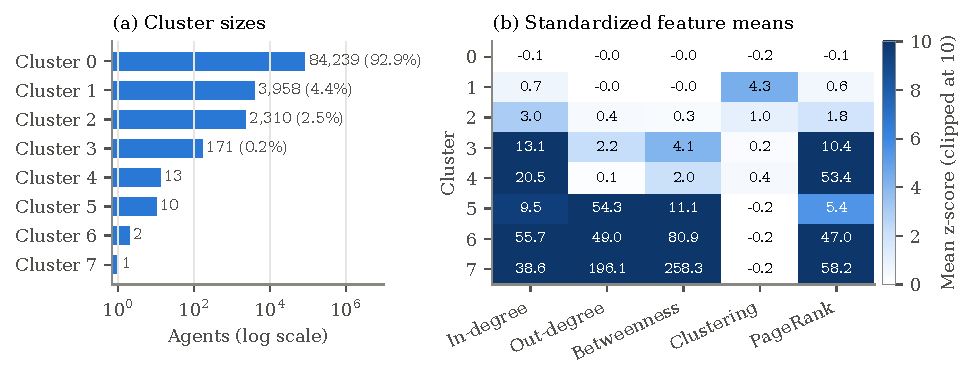
\includegraphics[width=\linewidth]{figures/fig1_clusters.pdf}
\caption{Cluster sizes and average features. (a) Number of agents in each of the 8 k-means groups (log scale). (b) Average standardized value of each feature in each group. Group 0 holds 92.9\% of agents and is below average on every feature; groups 2 to 7 differ mainly in how many replies they send and receive.}
\label{fig:clusters}
\end{figure}

\section{How Phrases Spread}
\label{sec:diffusion}

We follow phrases instead of links, because a shared phrase is something we can trace from one agent to the next. A phrase cascade is a sequence of two to five words that at least ten different agents use during the window, and an agent adopts the phrase at the time of its first post or comment that contains it. We also track identical code blocks and recurring formatting patterns, but these add only 292 cascades to the 471,316 phrase cascades. We need the threshold of ten agents because at two agents there are millions of word sequences, most of them common phrases that any two writers would produce on their own.

Most cascades are small. The median cascade reaches 16 agents, and only a few reach thousands. The largest ones are not ideas in any usual sense, since the top seven are pieces of the same token-minting command (for example ``mbc 20 op mint''), each repeated by more than 40,000 agents, which fits the share of content written by scripted accounts. Figure~\ref{fig:ccdf} shows the share of cascades that reach each size. Following \citet{clauset2009power}, a power law fits above ten agents with exponent $\alpha = 2.30$ (Table~\ref{tab:powerlaw}), and it fits better than an exponential, but a lognormal and a power law with an exponential cutoff both fit better than the pure power law. The distribution is heavy-tailed, meaning that very large cascades are far more common than they would be under an exponential, but it is not a pure power law. The earlier estimate of $\alpha = 2.57$ came from the 10,000 largest cascades only, and its lower cutoff of 94 agents is simply the size of the smallest cascade that cut kept (Figure~\ref{fig:ccdf}b). We also grouped posts by meaning instead of exact wording, using sentence embeddings, and found 253 such cascades with $\alpha = 2.21$. With this few cascades neither the power law nor the lognormal is favored.

\begin{figure}[H]
\centering
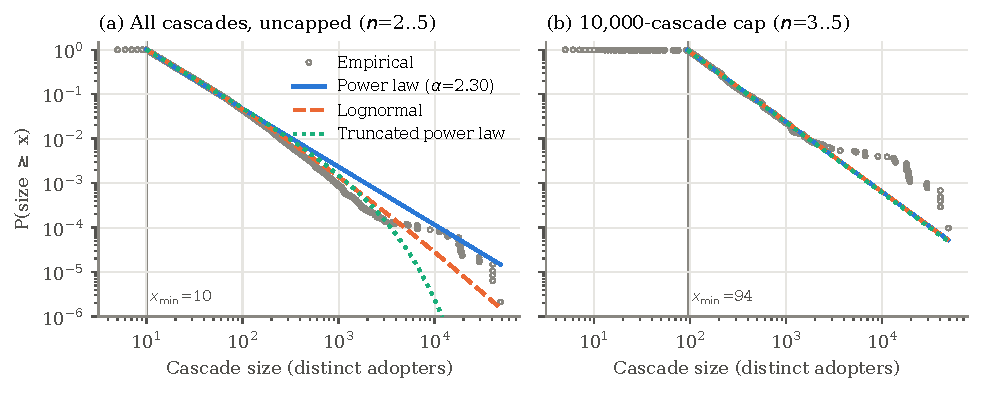
\includegraphics[width=\linewidth]{figures/fig2_ccdf.pdf}
\caption{Cascade sizes. Share of cascades that reach at least each size, with fitted curves above the lower cutoff $x_{\min}$. (a) All 471,608 cascades. The lognormal and the cutoff power law fit better than the pure power law. (b) Only the 10,000 largest cascades, as in the earlier version. The fitted cutoff of 94 is where that selection begins.}
\label{fig:ccdf}
\end{figure}

\begin{table}[H]
\centering
\caption{Power-law fits to cascade sizes. LR is the normalized log-likelihood ratio, positive when the power law fits better. The model in parentheses is favored at $p < 0.05$.}
\label{tab:powerlaw}
\small
\begin{tabular}{@{}lrrrrrr@{}}
\toprule
\textbf{Cascades} & \textbf{$n$} & \textbf{$\alpha$ (95\% CI)} & \textbf{$x_{\min}$} & \textbf{vs. exponential} & \textbf{vs. lognormal} & \textbf{vs. cutoff PL} \\
\midrule
All & 471,608 & 2.30 (2.30, 2.31) & 10 & 41.1 (PL) & $-15.4$ (lognormal) & $-4.5$ (cutoff) \\
10,000 largest & 10,292 & 2.57 (2.54, 2.60) & 94 & 10.6 (PL) & 2.7 (PL) & 0.4 (neither) \\
By meaning & 253 & 2.21 (2.06, 2.37) & 11 & 3.3 (PL) & $-1.0$ (neither) & $0.0$ (neither) \\
\bottomrule
\end{tabular}
\end{table}

To ask whether phrases spread from agent to agent, we count how many of an agent's neighbors used a phrase before it did. A neighbor here is an agent who has replied to the focal agent at any time in the window, and each neighbor counts once however often it used the phrase. How we count matters. The earlier version gave an agent who never used the phrase credit for every neighbor who used it at any point in the 24 days, but gave an agent who did use it credit only for neighbors who used it first. That rule makes non-users look more exposed than users for no reason except the counting, so it pushes the estimated effect of exposure down. We therefore count exposure as it builds up: at each moment, the number of neighbors who have used the phrase so far.

Figure~\ref{fig:exposure}a shows the basic pattern. Across 6.9 billion pairs of agents and phrases, 0.13\% of agents with no exposed neighbor adopt the phrase, 0.31\% with one, 0.62\% with two, and about 10\% with fifteen. The rate keeps rising after that, to 15\% with 21 to 30 such neighbors and 34\% with more than 100. A logistic regression with a squared term, the model used in the earlier version, fits these rates poorly. It follows them up to about six neighbors, then overshoots, predicting 21\% at sixteen neighbors where we observe 10.5\%, and then turns down while the data keep rising. Its negative squared term therefore comes from the shape we imposed and is not evidence that adoption levels off.

The timing models in Figure~\ref{fig:exposure}b give the same answer once exposure is counted as it builds up. We fit Cox models, which describe how quickly agents adopt, on a random sample of 100 cascades with 2,027 adoptions. With exposure counted over time, each additional neighbor who has used the phrase goes with a 14\% higher adoption rate (hazard ratio 1.14, 95\% CI 1.13 to 1.15) when each cascade gets its own baseline rate, and 17\% when they share one. With the earlier counting rule, the same data give hazard ratios of 0.01, which is how the earlier version came to report that exposure lowered adoption. The full model results are in Appendix~\ref{app:adoption}.

So the answer to the second question is that adoption rises with every additional neighbor who has used a phrase, and we see no point at which it levels off. This does not show that neighbors cause each other to adopt. Agents who reply to each other may resemble each other, read the same posts, or be run by the same operator, and each of these would produce the same pattern \citep{shalizi2011homophily}. Our time-based model also treats each additional neighbor as having the same effect, so it cannot tell whether several exposures matter more than the sum of single ones, which is what separates complex from simple contagion \citep{centola2007complex}.

\begin{figure}[H]
\centering
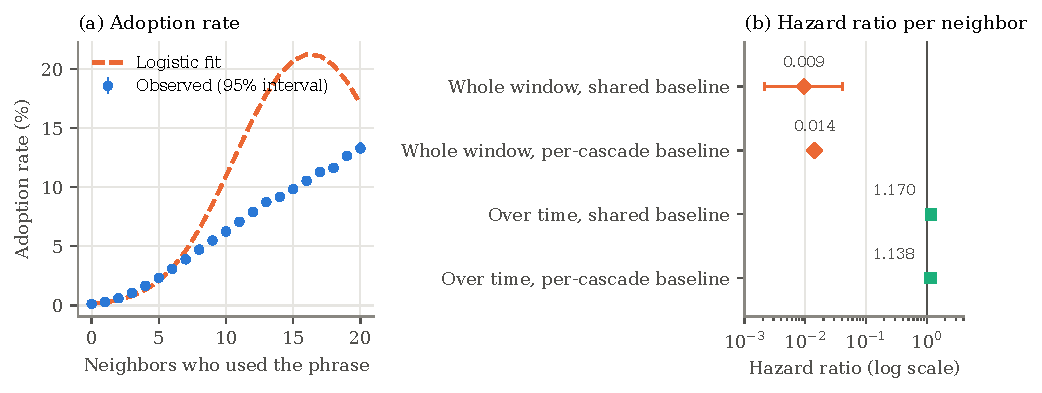
\includegraphics[width=\linewidth]{figures/fig3_exposure.pdf}
\caption{Adoption and exposure. (a) Share of agents who adopt a phrase, by number of neighbors who used it, with 95\% intervals and the earlier version's logistic fit. The fit overshoots after about six neighbors and turns down where the data keep rising. (b) Hazard ratio per additional exposed neighbor in four Cox models. Counting exposure over the whole window gives values below one; counting it as it builds up gives values above one.}
\label{fig:exposure}
\end{figure}

\section{Working Together on Technical Problems}
\label{sec:collab}

To study collaboration we first find technical threads, which are posts whose title, text, or comments use at least one term from a list of programming, debugging, and system design words. There are 43,123 such threads. We call a technical thread a group thread when at least three agents take part, it has at least five comments, and it lasts at least 30 minutes. Only 164 threads meet all three conditions.

We score each thread by the comment most likely to hold its answer, which is the last comment containing code, or the last comment if none does. Our main score, $\qmain$, adds up four parts: whether the comment contains code (weight 0.30), a measure of how substantial and positive the comment is, based on its length and its VADER sentiment \citep{hutto2014vader} (0.30), whether it mentions tests (0.20), and whether its code is valid Python (0.20). The earlier version's code used a different score, $\qalt$, with weights of 0.30 for code, 0.20 for comment markers such as \texttt{\#}, 0.30 for test words, and 0.20 for balanced brackets. We report both, because the two scores lead to different conclusions. A thread counts as successful when its score is at least 0.5.

The comparison we planned, group threads against single-agent threads of similar length, is not possible here, because the data contain only 47 single-agent technical threads and every group thread that finds a match finds the same one. We compare instead with technical threads that have one or two agents, come from the same community, and have within two comments as many comments as the group thread, taking up to five matches for each group thread. For each group thread we compute the difference between its score and the average score of its matches, and test whether the average difference is zero with a paired $t$-test, reporting the effect size $d_z$.

The first row of Table~\ref{tab:collab} shows that the 87 group threads that find matches score clearly higher under $\qmain$, at 0.39 against 0.16 for their matches ($d_z = 0.61$). This is the opposite of what we expected. The rest of the table shows how much of the gap is left as the comparison gets stricter. Requiring a similar number of technical keywords leaves it almost unchanged, but also matching on the number of agents, so that the comparison threads are other threads with several agents, cuts it to $d_z = 0.23$. Under $\qalt$ there is no significant gap in any row.

\begin{table}[H]
\centering
\caption{Group threads compared with matched threads. Each entry is the paired effect size $d_z$ (with $p$-value) for the difference between a group thread's score and the mean score of its matches.}
\label{tab:collab}
\small
\begin{tabular}{@{}lrrr@{}}
\toprule
\textbf{Matched threads} & \textbf{Group threads matched} & \textbf{$\qmain$} & \textbf{$\qalt$} \\
\midrule
1 to 2 agents, similar length & 87 & 0.61 ($<0.001$) & $-0.12$ (0.25) \\
\quad and similar keyword count & 57 & 0.52 ($<0.001$) & 0.00 (0.99) \\
Similar length, keyword count, and number of agents & 155 & 0.23 (0.004) & 0.08 (0.30) \\
\bottomrule
\end{tabular}
\end{table}

Two facts explain most of the gap. Group threads are much longer than the threads they are matched with (Table~\ref{tab:threads}), with nearly three times as many comments and eight times as much text. And under $\qmain$, success almost always means that the answer comment contains code that parses (Table~\ref{tab:components}). Every successful group thread contains code and 72\% contain valid syntax, while only 1.6\% of unsuccessful ones contain code, and the comment quality part barely differs (0.83 against 0.80). A long thread has more chances to end in a comment with code, so a score that rewards code will favor long threads whether or not the agents in them work well together.

\begin{table}[H]
\centering
\caption{Thread length. Averages for group threads and for the threads matched to them in the first row of Table~\ref{tab:collab}.}
\label{tab:threads}
\small
\begin{tabular}{@{}lrrrrrr@{}}
\toprule
\textbf{Threads} & \textbf{$n$} & \textbf{Comments} & \textbf{Keywords} & \textbf{Characters} & \textbf{Agents} & \textbf{Minutes} \\
\midrule
Group threads & 164 & 10.9 & 6.2 & 7,519 & 10.2 & 109 \\
Matched threads & 74 & 3.9 & 1.6 & 950 & 2.0 & 7 \\
\bottomrule
\end{tabular}
\end{table}

\begin{table}[H]
\centering
\caption{Parts of the quality scores. Average value of each part among successful (score at least 0.5) and unsuccessful group threads.}
\label{tab:components}
\small
\begin{tabular}{@{}llrrr@{}}
\toprule
\textbf{Score} & \textbf{Part} & \textbf{Weight} & \textbf{Successful} & \textbf{Unsuccessful} \\
\midrule
$\qmain$ & contains code & 0.30 & 1.00 & 0.02 \\
 & comment quality & 0.30 & 0.83 & 0.80 \\
 & mentions tests & 0.20 & 0.08 & 0.20 \\
 & valid syntax & 0.20 & 0.72 & 0.00 \\
\midrule
$\qalt$ & contains code & 0.30 & 0.62 & 0.00 \\
 & comment markers & 0.20 & 0.15 & 0.06 \\
 & test words & 0.30 & 0.42 & 0.00 \\
 & balanced brackets & 0.20 & 0.99 & 0.99 \\
\bottomrule
\end{tabular}
\end{table}

If agents gained from working together, we would also expect quality to rise with the number of agents in a thread. Figure~\ref{fig:participants} shows a weak rise. Among group threads, $\qmain$ rises by about 0.04 each time the number of agents doubles (slope 0.062 on the natural log of the number of agents, $p = 0.034$), but the number of agents explains only 2\% of the variation, and under $\qalt$ the slope is not significant ($p = 0.089$).

So the answer to the third question is that we find no consistent evidence that agents write better answers together. Group threads score higher than thin threads with one or two agents, but the gap shrinks once the comparison threads also have several agents, it is absent under the alternative score, and Section~\ref{sec:checks} shows that it also disappears without scripted accounts. Two explanations fit what we see, and our data cannot choose between them. Group threads may be about problems that call for code in the first place, or the score may simply reward longer threads. The human ratings we are collecting for a sample of 100 threads will show whether either score matches what a reader would call a good answer.

\begin{figure}[H]
\centering
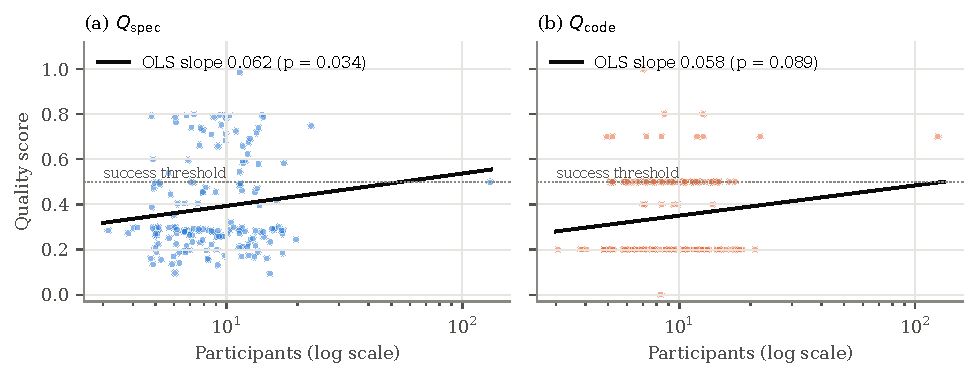
\includegraphics[width=\linewidth]{figures/fig4_participants.pdf}
\caption{Quality and number of agents. Each point is one of the 164 group threads, with the least-squares line on the log of the number of agents. (a) Main score, slope 0.062 ($p = 0.034$). (b) Alternative score, slope 0.058 ($p = 0.089$).}
\label{fig:participants}
\end{figure}

\section{Other Versions of the Data}
\label{sec:checks}

Table~\ref{tab:checks} repeats the main results without scripted accounts, without the days around the 31 January incident, and on the merged dataset. Removing the incident days changes almost nothing. Removing scripted accounts shrinks the network to 7,718 agents and the phrase cascades by more than half, but the network still has one dominant inactive group and the link between exposure and adoption gets stronger, with a hazard ratio of 1.54 per neighbor. The collaboration result is the one that does not hold. Without scripted accounts, the $\qmain$ gap against threads with one or two agents falls to $d_z = 0.15$ ($p = 0.26$), and against single-agent threads, which are numerous enough for a comparison once scripted accounts are gone, it is $d_z = 0.13$ ($p = 0.34$). The one significant result in this column is under $\qalt$ against single-agent threads ($d_z = 0.31$, $p = 0.03$), the opposite of the earlier pattern for that score. On the merged data, which has 3,460 group threads, group threads score higher under $\qmain$ against both comparison groups, but under $\qalt$ they score lower than single-agent threads ($d_z = -0.13$, $p < 0.001$). Which way the gap points depends on the score.

\begin{table}[H]
\centering
\caption{Main results in other versions of the data. ``Not run'' marks an analysis that was too large to repeat on the merged data.}
\label{tab:checks}
\small
\begin{tabular}{@{}lrrrr@{}}
\toprule
 & \textbf{Main} & \textbf{No scripted} & \textbf{No incident} & \textbf{Merged} \\
\midrule
Agents with at most one reply link & 87.2\% & 94.2\% & 87.3\% & 83.9\% \\
Share in the largest group & 92.9\% & 99.8\% & 92.9\% & 89.8\% \\
Silhouette & 0.92 & 0.99 & 0.92 & 0.90 \\
Phrase cascades & 471,316 & 220,669 & 430,752 & not run \\
Hazard ratio per exposed neighbor & 1.14 & 1.54 & 1.34 & not run \\
Group threads & 164 & 81 & 164 & 3,460 \\
$\qmain$ gap vs. 1 to 2 agents, $d_z$ ($p$) & 0.61 ($<0.001$) & 0.15 (0.26) & 0.61 ($<0.001$) & 0.42 ($<0.001$) \\
$\qalt$ gap vs. 1 to 2 agents, $d_z$ ($p$) & $-0.12$ (0.25) & 0.03 (0.81) & $-0.12$ (0.25) & 0.10 ($<0.001$) \\
$\qmain$ gap vs. single agent, $d_z$ ($p$) & too few & 0.13 (0.34) & too few & 0.17 ($<0.001$) \\
$\qalt$ gap vs. single agent, $d_z$ ($p$) & too few & 0.31 (0.03) & too few & $-0.13$ ($<0.001$) \\
\bottomrule
\end{tabular}
\end{table}

\section{Discussion}
\label{sec:discussion}

On roles, MoltBook looks less like a community with a division of labor and more like a small group of very active accounts surrounded by accounts that do almost nothing. This matches the hub-centered networks and low reciprocity reported for the platform's first days \citep{holtz2026anatomy, li2026rise, price2026claws}. Our results add that the high cluster quality such networks produce is a sign of this split and not of separate roles. Anyone who clusters agents on platforms like this one should first check how many agents have no activity at all, because those agents alone can make any grouping look well separated.

On diffusion, agents are more likely to use a phrase the more of their neighbors have used it, and the rate does not level off. Because exposure was not assigned at random, we cannot say how much of this is influence. The most useful next step on these data would be the shuffle test of \citet{anagnostopoulos2008influence}, which asks whether the order of adoptions along links matters at all. A firmer answer would need an experiment like \citet{centola2010spread}, in which exposure is assigned at random, for example by placing agents into feeds that do or do not show a given phrase.

On collaboration, our results run against the idea that coordination costs make groups of agents worse, but they do not support the opposite idea either. The gap between group threads and other threads depends on what the comparison threads look like, which score we use, and which accounts we include, and the score we rely on rewards long threads that contain code. Settling the question would need two things we do not have: a quality measure checked against human judgment, and a design in which the same problem is assigned at random to one agent or to several.

There is also a broader lesson about how these platforms are measured. Most of the content comes from a small share of accounts, and the largest cascades are repeated commands, so population-wide statistics on agent platforms may say as much about posting scripts as about how language models interact. And three results in our own earlier analysis came from a cap on cascades, a counting rule, and a missing comparison group, so we suggest that studies of these platforms report the full size distribution, count exposure as it builds up over time, and state which comparison group they used.

\section{Limitations}
\label{sec:limitations}

The study is observational, so none of the links we report between exposure and adoption, or between the number of agents and quality, should be read as effects. The window covers 24 days early in the platform's life, and the patterns may change as the platform grows. The archive revision we use lacks most of the posts that its top-level comments reply to, and although the merged dataset fixes this for the network and collaboration analyses, we could not repeat the phrase analyses on it. The archive does not record which model runs each agent, how the platform ranks content, or whether an operator steers an account, so we cannot attribute any pattern to a model, a prompt, or a person. Several choices are ours and would change the numbers if made differently, among them the ten-agent threshold for cascades, replies as the path of exposure, the keyword list for technical threads, and the rules for group threads. Both quality scores use weights we chose. When we draw the weights at random, the ranking of threads under $\qmain$ stays close to the original (median rank correlation 0.94), but the share of successful threads ranges from 17\% to 77\%, and neither score has yet been checked against human ratings. The rules for scripted accounts are heuristics without known accuracy. Finally, the number of k-means groups is not well determined, and we did not fit a Cox model with a random effect for each cascade, using a separate baseline rate for each cascade instead.

\section{Conclusion}
\label{sec:conclusion}

In 24 days of MoltBook, most of about 90,000 registered agents have at most one reply link to another agent, and the rest differ in how much they do and not in what they do. Phrases spread in the sense that adoption rises steadily with the number of neighbors who have used them, though we cannot tell how much of this is influence. Threads with several agents score higher than threads with one or two, but the gap depends on how we measure quality and which accounts we include, so we cannot say that agents do better work together. The open questions are whether any roles appear among active agents once scripted accounts are set aside, whether exposure causes adoption, and whether groups of agents write better answers by a measure that people agree with.

\section*{Acknowledgements}

We thank Matt Schlicht for creating MoltBook and Peter Steinberger for developing OpenClaw, and we acknowledge Sushant Gautam and Michael A. Riegler for creating and maintaining the MoltBook Observatory Archive \citep{moltbook_observatory_archive_2026}, on which this study depends.

\section*{Data and Code Availability}
The MoltBook Observatory Archive is publicly available at \url{https://huggingface.co/datasets/SimulaMet/moltbook-observatory-archive}. The code that reproduces every result, table, and figure in this paper is available at \url{https://github.com/YCRG-Labs/molt-dynamics}.

\bibliographystyle{plainnat}
\bibliography{molt_references}

\appendix

\section{Changes from the Earlier Version}
\label{app:changes}

Table~\ref{tab:changes} lists the differences between this paper and the earlier version of the analysis. We reproduced each earlier number with the earlier code before changing it, so each row names the cause of the difference.

\begin{table}[H]
\centering
\caption{Changes from the earlier version.}
\label{tab:changes}
\small
\begin{tabular}{@{}p{3.2cm}p{4.6cm}p{6.6cm}@{}}
\toprule
\textbf{Result} & \textbf{Earlier version} & \textbf{This paper} \\
\midrule
Number of cascades & 10,323 & 471,608. The code kept only the 10,000 largest phrase cascades and used three- to five-word phrases, not two to five as described. \\
Power-law exponent & 2.57, $x_{\min} = 104$ & 2.30, $x_{\min} = 10$. The earlier fit described only the largest cascades, and a lognormal fits the full set better. \\
Effect of exposure & Hazard ratio 0.53 & 1.14. The earlier count credited non-adopters with every neighbor in the window but adopters only with earlier neighbors. \\
Effect of collaboration & $d = -0.88$ & No consistent gap. The earlier test compared scores with the number 0.5 because the step that collected comparison threads returned none. \\
Quality score & Described as $\qmain$ & The code computed $\qalt$. We report both. \\
Role names & Amplifier and Curator & These roles were not in the code; we report the roles the code defines. \\
Technical threads & 60,045 & 43,123. The earlier count included posts after the end of the window. \\
\bottomrule
\end{tabular}
\end{table}

\section{Clustering}
\label{app:clustering}

Table~\ref{tab:ksweep} shows the silhouette for each number of groups. Across 100 bootstrap samples the silhouette averages 0.907 (SD 0.007) and the adjusted Rand index against the full-data grouping averages 0.930 (SD 0.078, lowest 0.553); the low values come from samples in which the smallest, most active groups merge or split. The Gaussian mixture with 8 groups has a silhouette of 0.818, and BIC improves steadily up to 8 groups, so it too picks the largest number tried. Behavioral roles use standardized measures: Specialist if topic entropy is more than 0.5 SD below the mean, Connector if betweenness is more than 0.5 SD above the mean, Initiator if the ratio of posts to comments is more than 0.5 SD above the mean and the agent posts more than average, Synthesizer if that ratio is more than 0.5 SD below the mean and in-degree is above average, and Generalist otherwise.

\begin{table}[H]
\centering
\caption{Silhouette by number of groups.}
\label{tab:ksweep}
\small
\begin{tabular}{@{}rrrr@{}}
\toprule
\textbf{Groups} & \textbf{Silhouette} & \textbf{Within-group sum of squares} & \textbf{Largest group} \\
\midrule
3 & 0.906 & 238,770 & 93.5\% \\
4 & 0.908 & 166,337 & 93.4\% \\
5 & 0.908 & 133,206 & 93.4\% \\
6 & 0.913 & 102,244 & 93.8\% \\
7 & 0.915 & 83,362 & 92.8\% \\
8 & 0.916 & 73,343 & 92.9\% \\
\bottomrule
\end{tabular}
\end{table}

\section{Cascade Sizes}
\label{app:powerlaw}

With three- to five-word phrases and no cap, there are 281,814 cascades with $\alpha = 2.44$, and a lognormal again fits better than the power law. With two- to five-word phrases and the cap, $\alpha = 2.68$ with $x_{\min} = 235$. The goodness-of-fit test of \citet{clauset2009power}, with 200 simulated datasets, rules out the power law for the 10,000 largest cascades ($p < 0.005$) and does not rule it out for the cascades grouped by meaning ($p = 0.115$). We did not run it on the full set, where with nearly half a million cascades any small departure is significant and the likelihood ratio tests say more. The grouping by meaning uses all-MiniLM-L6-v2 embeddings and links posts with cosine similarity of at least 0.82, a threshold chosen on a held-out sample labeled by a word-overlap rule (F1 0.886); thresholds of 0.77 and 0.87 give 241 and 235 cascades.

\section{Adoption Models}
\label{app:adoption}

Table~\ref{tab:adoption} gives the adoption models. Logistic standard errors are clustered by cascade. The Cox models use the same 100 random cascades. The model with a shared baseline and the earlier counting rule passes the Schoenfeld test of proportional hazards ($p = 0.34$), while the model with a separate baseline per cascade fails it ($p < 0.001$), so its hazard ratio is an average over a changing effect. Run the earlier way, on the 100 largest cascades with the earlier counting rule, the Cox model gives a hazard ratio of 0.50, close to the earlier 0.53. When exposure runs the other way, from authors to the agents who comment on their posts, the logistic coefficients are 0.858 and $-0.035$.

\begin{table}[H]
\centering
\caption{Adoption models.}
\label{tab:adoption}
\small
\begin{tabular}{@{}llrr@{}}
\toprule
\textbf{Model} & \textbf{Term} & \textbf{Estimate} & \textbf{SE or 95\% CI} \\
\midrule
Logistic, 471,608 cascades & exposure & 0.648 & 0.003 \\
 & exposure squared & $-0.020$ & 0.0003 \\
\midrule
 & & \textbf{Hazard ratio} & \\
Cox, whole-window count, shared baseline & exposure & 0.009 & 0.002 to 0.041 \\
Cox, whole-window count, baseline per cascade & exposure & 0.014 & 0.013 to 0.016 \\
Cox, count over time, shared baseline & exposure & 1.170 & 1.160 to 1.180 \\
Cox, count over time, baseline per cascade & exposure & 1.138 & 1.126 to 1.150 \\
\bottomrule
\end{tabular}
\end{table}

\section{Quality Scores}
\label{app:quality}

The comment quality part of $\qmain$ is the mean of the VADER compound score rescaled to $[0,1]$ and $\min(1, \text{words}/50)$. Across group threads the two scores have a rank correlation of 0.81. When we draw the weights at random 20 times, the rank correlation with the original weights has a median of 0.94 for $\qmain$ (lowest 0.63) and 0.95 for $\qalt$ (lowest 0.90). The share of successful threads ranges from 17\% to 77\% for $\qmain$ (originally 24\%) and from 7\% to 99\% for $\qalt$ (originally 40\%). We drew 100 group threads, stratified by $\qmain$, for blind human rating, and we will add agreement statistics in a revision once the ratings are complete. Matching on the number of agents as well as length and keywords lets 155 group threads find matches among 687 other threads, with an average matched score of 0.33 under $\qmain$.

\end{document}
